\documentclass[en,hazy,blue,screen,14pt]{elegantnote}
\usepackage[T1]{fontenc}
\usepackage[latin9]{inputenc}
\usepackage{babel}
\usepackage{float}
\usepackage{textcomp}
\usepackage{amsmath,amsfonts,amssymb}
\usepackage{amsthm}
\usepackage{graphicx}
%\usepackage[ruled,vlined]{algorithm2e}
\PassOptionsToPackage{normalem}{ulem}
\usepackage{ulem}
\usepackage{mathtools}
\usepackage{url}
\usepackage{hyperref}
\usepackage{algorithm, algpseudocode}

\renewcommand\qedsymbol{$\blacksquare$}
\DeclarePairedDelimiter{\ceil}{\lceil}{\rceil}
\newcommand\tab[1][1cm]{\hspace*{#1}}
\newenvironment{claim}[1]{\par\noindent\underline{Claim:}\space#1}{}
\newenvironment{claimproof}[1]{\par\noindent\underline{Proof:}\space#1}{\hfill $\blacksquare$}
\renewcommand{\algorithmicrequire}{\textbf{Input:}}
\renewcommand{\algorithmicensure}{\textbf{Output:}}

\title{Class Notes\\CIS 502 Analysis of Algorithm\\6-Network Flows}
\author{Da Kuang}
\institute{University of Pennsylvania}
% \version{1.00}
\date{}

\begin{document}

\maketitle
\newpage
% \input{}
\section{Network Flow}
\subsection{Problem Formulation}
Given:
\begin{itemize}
	\item A directed graph $G = (V, E)$
	\item A capacity function $c: E \rightarrow \mathbb{Z}^+$
	\item A source $s$ and a sink $t$.
\end{itemize}
Find:
\begin{itemize}
	\item A flow $f: E \rightarrow \mathbb{R}$ such that
		\begin{itemize}
			\item Capacity constraints: $\forall e \in E, ~f(e) \le c(e)$.
			\item Non-negativity: $\forall e \in E, ~f(e) \ge 0$.
			\item Conservation constrains: $\forall v \in V - \{s, t\}, ~\sum_{(u,v) \in E} f(u,v) = \sum_{(v, u) \in E}f(v,u)$
		\end{itemize}
	\item To maximize net flow out of $s$:
	\[|f| = \sum_{(s,u) \in E} f(s, u) - \sum_{(u,s) \in E} f(u,s)\]
\end{itemize}
The following is an example of network flow:
\begin{figure}[H]
	\centering
	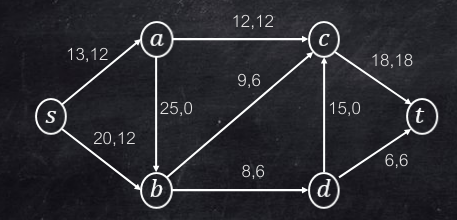
\includegraphics[width=0.5\textwidth]{fig/flow.png}
\end{figure}
The first number on the edge is the capacity of the edge. The second number is the flow on each edge. The flow value $|f| = 24$.

\subsection{Residual Graph}
After we have built up a flow $f$, we construct a residual graph $G_f$ that shows all the edges on which we can still send flow.

Rules for constructing residual graph:
\begin{itemize}
	\item If $G$ has edge $(u, v)$ with $f(u, v) < c(u, v)$ then $G_f$ has edge $(u, v)$ with capacity $c(u, v) - f(u, v)$. (Excess capacity of $(u,v)$)
	\item If $G$ has edge $(u, v)$ with $f(u, v) > 0$, then $G_f$ has edge $(v, u)$ with capacity $f(u, v)$. (Amount of flow can be removed from $(u,v)$)
\end{itemize}

An example is as following. Note that edges that were ``saturated'' do not exist in forward direction.
\begin{figure}[H]
	\centering
	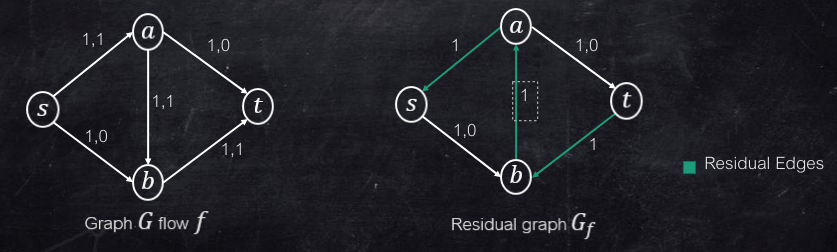
\includegraphics[width=0.6\textwidth]{fig/gf.png}
\end{figure}

\subsection{Adding Two Flow}
If $f_1$ and $f_2$ are two flows, we can add them together to get a flow $f$ as follows:
\begin{itemize}
	\item For an edge $(u,v)$, $f(u,v) = f_1(u,v) + f_2(u,v)$.
	\item If $f_1$ has a positive flow on edge $(u, v)$, and $f_2$ on edge $(v, u)$ in residual graph, then $f(u,v) = f_1(u,v) - f_2(v,u)$.
\end{itemize}
Note that the flows will be non-negative as long as $f_1(u,v) \ge f_2(v, u)$ in second case. It will always be true because we give the edge $(v, u)$ a capacity of $f_1(u, v)$ in $G_{f_1}$.



\section{Finding Max Flow: Ford-Fulkerson Algorithm}
Algorithm:
\begin{itemize}
	\item Start with the all-zero flow
	\item Let current flow be $f$.
	\item Construct residual graph $G_f$.
	\item While there is a path from $s$ to $t$ in $G_f$.
	\begin{itemize}
		\item Find a flow $f_1$ on such a path (limited by min capacity on path)\item Set new flow to be $f = f + f_1$
		\item Construct new residual graph $G_f$.
	\end{itemize}
\end{itemize}

Easy to see that the algorithm only produces feasible flows.

The following is an example. It turns out that the algorithm is not so fast and it could repeatedly take a path involving the middle edge and only be able to augment the flow value by 1 per iteration.
\begin{figure}[H]
	\centering
	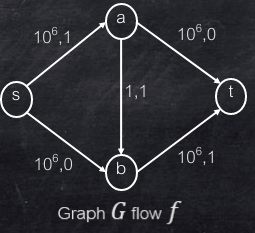
\includegraphics[width=0.3\textwidth]{fig/runtime.png}
\end{figure}
It will take 2-million iterations to arrive at the flow value of 2 million. This is not efficient because capacity $n$ can be represented by $\log n$ input bits. But if the capacities are small integers, then this algorithm is okay.


\section{Correctness}
\subsection{s-t cuts in flow networks}

In graph, cuts are defined by dividing vertices into two parts and consist of the edges with one endpoint in each part. In flow networks s-t cuts are similar.

\begin{definition}
	An $s - t$ cut is defined by partitioning $V$ into $S$ and $T$, with $s \in S$, and $t \in T$.
\end{definition}

The difference between a cut in a graph and a cut in a flow network is as following: for a cut in a flow network, source $s$ and terminal $t$ must belongs to different sets.

\begin{definition}
	Forward edges are edges from set $S$ to set $T$. Backward edges are edges from set $T$ to set $S$.
\end{definition}
An example is as follows:
\begin{figure}[H]
	\centering
	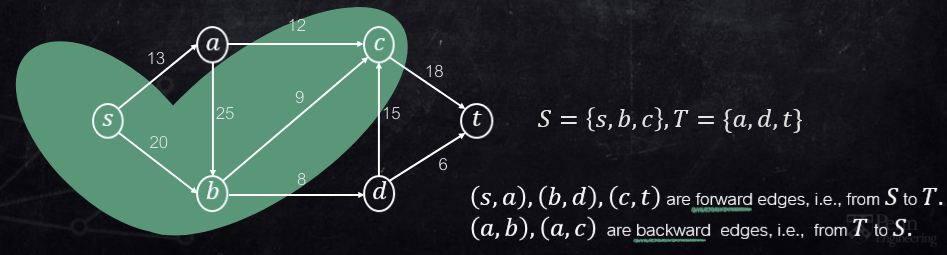
\includegraphics[width=0.8\textwidth]{fig/cut.png}
\end{figure}
\subsubsection{Notes}
For each cut $(S, T)$, any flow going from $s$ to $t$ must go from $S$ to $T$.

Because of conservation of flow, we can prove that $|f|$, the net flow out of $S$, is also the flow across any cut $(S, T)$ and the net flow into $t$.
\subsubsection{Example}
Imagine a city with a river running through it and only a few bridges across the river. The rate of traffic flow from the left bank to the right bank is limited by the rate that the bridges can bear.

Bridges form a cut. Removing them separates the left bank from the right; their capacity is a constraint on the amount of flow you can have.
\subsubsection{Capacity of a Cut}
The capacity of an $s-t$ cut $(S, T)$ should represent the maximum net flow you can send across the cut. Net flow across $(S, T)$ is sum of flows on forward edges minus sum of flows on backward edges. To send maximum net flow, must saturate the forward edges, and have 0 flow on the backward edges.
\begin{definition}
	The \textbf{capacity} of a cut is defined as the sum of the capacities of the forward edges of the cut.
\end{definition}

In the above example, the capacity of $s-t$ cut is $13 + 8 + 18 = 39$.

\subsubsection{Cut capacities and flow values}
Capacity of any $s-t$ cut is an \textbf{upper bound} on flow value of any flow. Cuts with small capacities are \textbf{bottlenecks}, like the bridges in a city. The minimum cut is the cut with the smallest capacity and the flow value must be no greater than this capacity.

\subsubsection{Correctness of Ford-Fulkerson}
\paragraph{Main idea:} If there are no paths from $s$ to $t$ in $G_f$, we know that Ford-Fulkerson terminates with flow $f$. So let us define a cut by letting $S$ be the set of all vertices reachable from $s$ in $G_f$. Let $T$ be the complementary set. We will show that the flow across this cut, and hence $|f|$ must be equal to the capacity of the cut, thereby proving that we have a max flow.

When Ford-Fulkerson terminates, we have an $s-t$ cut $(S-T)$ because $t$ is not
reachable from $s$ in $G_f$.

In the following example is a graph of net flow, there are two kinds of edge $(u,v)$ and $(x,y)$. The former is from $S$ to $T$ and the latter is from $T$ to $S$.
\begin{figure}[H]
	\centering
	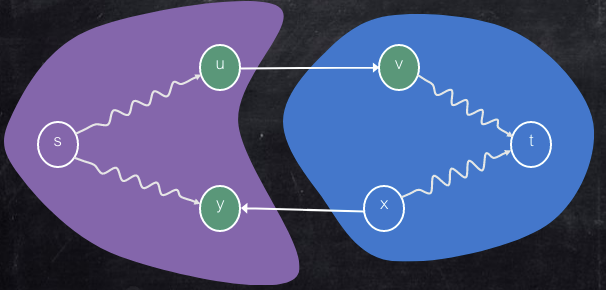
\includegraphics[width=0.5\textwidth]{fig/cut-2.png}
\end{figure}
\begin{itemize}
	\item Why did the forward edge $(u,v)$ not exist in $G_f$?
	\begin{itemize}
		\item Naively, if $(u, v)$ is a forward edge, then $v$ is reachable from $s$ and it should be in set $S$. In fact, it is because that the cutting edges carries as much flow as their capacity.
	\end{itemize}
	\item Why did backward edge $(y, x)$ not exist in $G_f$?
	\begin{itemize}
		\item If the back edge exist, $x$ would have been in $S$. Therefore, edge $(x, y)$ carries $0$ flow.
	\end{itemize}
\end{itemize}

So when Ford-Fulkerson stops, we have a cut (where $S$ contains vertices reachable from $S$) such that:
\begin{itemize}
	\item All forward edges are carrying as much flow as their capacity.
	\item All backward edges are carrying 0 flow.
\end{itemize}
Therefore, the flow across $(S, T)$ = cap$(S, T)$. Moreover, the flow across $(S, T) = |f|$.

Thus, the current flow is equal to the capacity of $(S, T)$ and then it must be optimal. Incidentally, we have found a min-cut, namely, $(S, T)$.

\subsection{Run Time Analysis}
Each iteration of the while loop:

\begin{itemize}
	\item Construct a residual graph: $O(m)$, where $m$ is the number of edges.
	\item Find a path from $s$ to $t$ in residual graph: $O(m)$ by dfs or bfs.
	\begin{itemize}
		\item Such a path is an augmenting path, because it augments the flow value.
	\end{itemize}
	\item Add the flow on this path to current flow: $O(m)$.
\end{itemize}

Number of iterations:
\begin{itemize}
	\item If all capacities are integers, each augmentation increases $|f|$ by at least 1.
	\item Maximum flow value is no more than the sum of capacities of edges leaving $s$.
	\item If we call this sum $C$, we have at most $C$ augmentations.
\end{itemize}

Total running time is $O(mC)$.











\section{Max-FLow-Min-Cut-Theorem}
The preceding proof proves the correctness of Ford-Fulkerson. It also proves the max-flow-min-cut theorem.

\begin{theorem}
	In a flow network, the value of maximum flow is equal to the capacity of the minimum cut.
\end{theorem}

This is an important theorem and an example of a phenomenon called duality. It means that maximum value of something is equal to the minimum value of some other thing.
\section{Efficient Max Flow Algorithm: Capacity Scaling}
\begin{definition}
	\textbf{Capacity of an $s-t$ path} in $G_f$ is the capacity of the minimum capacity edge on the path.
\end{definition}

Modification to Ford-Fullerson Algorithm: augment along path of high capacity. We will not pushing ourselves by looking for the path with highest capacity since that might take too much time. Instead, we develop a strategy to find a path with reasonable high capacity by introducing a threshold $\Delta$. As long as possible, we augment along path of capacity at least $\Delta$. When no such path available, set $\Delta = \Delta / 2$.
\subsection{The Range of Delta}
So what is the highest/first $\Delta$ to consider: the largest power of 2 $\le$ capacity of some edge of leaving the source. We only consider this $\Delta$ because if we make $\Delta$ twice as large as this, then you will find no edge from the source have such capacity and therefore you will find no augmenting path.

On the other hand the smallest/last $\Delta$ to consider is 1. It means we considering all paths.
\subsection{Algorithm}
How to find augmenting path in the residual graph with capacity $\ge \Delta$?

Suppose you have a path with capacity at least $\Delta$ in the $G_f$ as following. 
\begin{figure}[H]
	\centering
	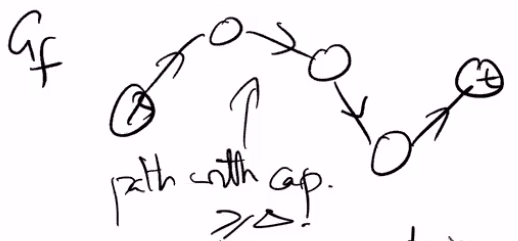
\includegraphics[width=0.5\textwidth]{fig/path-gf.png}
\end{figure}
Every edge on the path must has capacity $\ge \Delta$. Then we can define a subset of residual of graph called $G_f(\Delta)$, consisting only of edges with capacity $\ge \Delta$. Any path in $G_f(\Delta)$ from $s$ to $t$ will have capacity $\ge \Delta$.

Algorithm:
\begin{itemize}
	\item Start with 0 flow. Set $\Delta$ as described earlier. 
	\item Construct $G_f(\Delta)$.
	\item While there is an augmenting path in $G_f(\Delta)$, argument $f$ along this path. Reconstruct $G_f(\Delta)$ for the new flow and repeat.
	\item If there is no such path then set $\Delta = \Delta / 2$ and back to step 2 until $\Delta = 1$.
\end{itemize}

\subsection{Correctness}
\paragraph{Main Idea} Proof is same as the proof for Ford-Fulkerson's correctness. If you look at the new algorithm, it checks all the paths that Ford-Fulkerson uses. Even if it does not success finding the path when $\Delta$ has a high value, by the time $\Delta = 1$ you basically looking for all the augmenting paths. So you will find any the paths that exist.
\begin{definition}
	A phase of the algorithm is defined by a value of $\Delta$. So the number of phases is $O(\log C)$.
\end{definition}

How many augmentation can happen in each phase? 

When the $\Delta$-phase terminate we are ``pretty close'' to the optimal flow value. To quantify ``pretty close'', we make the following definition. 

\begin{definition}
	Let $f^*$ be the max flow. $|f^*|$ is the flow value of $f^*$. Let $f_{\Delta}$ be the flow at the end of the $\Delta$-phase. 
\end{definition}

\begin{theorem}
	$|f_{\Delta}| \ge |f^*| -m\Delta$, where $m$ is the number of edges in $G$.
\end{theorem}
\begin{proof}
	Consider the cut in $G_f(\Delta)$ at the end of the $\Delta$-phase, where $S$ consist of vertices reachable from $s$ in $G_f$ and $T$ consist of the others.
	\begin{figure}[H]
		\centering
		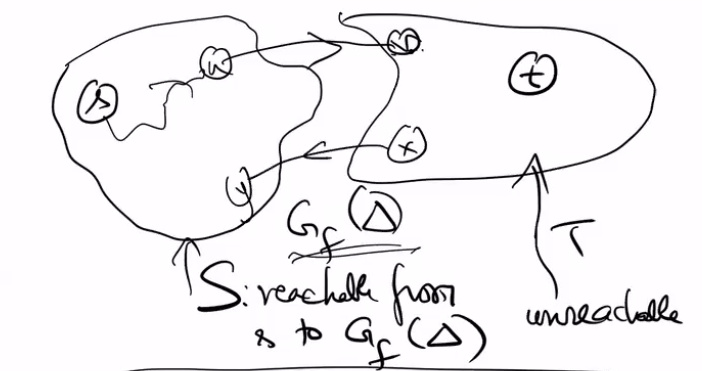
\includegraphics[width=0.6\textwidth]{fig/gf-delta.png}
	\end{figure}
	Look at this cut in the original graph $G$. Consider $u \in S$ and $v \in T$. If $(u, v)$ has residual capacity $\ge \Delta$. Then $(u, v)$ would have been present in $G_f(\Delta)$. This cannot happen because if $(u, v)$ has been present in $G_f(\Delta)$ then we are able to reach $u$ from $G_f(\Delta)$. If $(u, v)$ has residual capacity in $G_f(\Delta)$ then $v$ would be reachable as well. It is a contradiction because $v$ is actually not reachable from $S$ in $G_f(\Delta)$. .
	
	Therefore, $f(u,v) \ge c(u, v) - \Delta$. This is the only way that this edge would have residual capacity less than $\Delta$. 
	
	Now consider the edge $(x, y)$ in the back direction in the origin graph $G$, where $x \in T$ and $y \in S$. If $f(x, y) \ge \Delta$, then $(y, x)$ would have been present in $G_f(\Delta)$ with capacity $\ge \Delta$. It is also not possible since $x$ is not reachable. 
	
	Therefore, all backward edges carry at most flow $\Delta$.
	
	Based on the above facts, 
	\begin{align*}
		\text{net flow cross this cut} 
		\ge& \text{capacity of cut} - \Delta \times \text{(the number of edges across the cut)}\\
		\ge& \text{capacity of cut} - \Delta \times \text{(the number of edges in the graph)}
	\end{align*}
	
	Moreover, it is known that the capacity of cut is the upper bound of $|f^*|$. Therefore,
	
	\[|f_{\Delta}| \ge |f^*| - m\Delta\]	
\end{proof}
Based on the theorem, if we go to the next phase, $G_f(\frac{\Delta}{2})$, every augmentation increases the flow by at least $\frac{\Delta}{2}$. 

A phase starts with flow $f_{\Delta}$ can have at most $2m$ augmentation before flow value exceeds $|f^*|$. So for every phase, the number of augmentation is at most $2m$. Total number of augmentation across all phases $ = O(m \log C)$.


\subsection{Run Time Analysis}
How long does each augmentation take? 

We can construct $G_f(\Delta)$ in $O(m+n)$ time. DFS(or BFS) starting at $s$ will find an augmenting path to reach $t$ in $O(m+n)$ time if such a path exist. Overall running time is $O(m^2\log C)$.



\section{Appliction: Bipartite Matchings}
\subsection{Matching}
Matching in an undirected graph $G=(V, E)$ is subset $M \subset E$ such that each vertex $v$ has at most one edge in $M$ touching it. In this way, we are pairing up vertices so each vertex can get paired to at most one of the vertex or to none of them.

Here is an example as follows:

\begin{figure}[H]
	\centering
	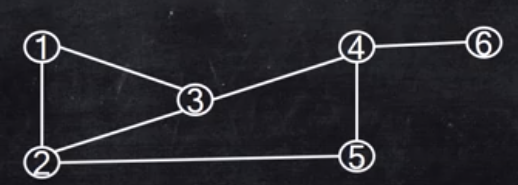
\includegraphics[width=0.5\textwidth]{fig/match.png}
\end{figure} 

In the example, $\{(1, 2), (4, 5)\}$ is a matching with 2 edges in it. $\{(1, 3), (2, 5), (4, 6)\}$ is another matching with 3 edges.

\subsection{Bipartite Graph}
Bipartite graphs are graphs $G = (V, E)$ where $V$ can be partitioned into $V_1$ and $V_2$ so that all edges go between $V_1$ and $V_2$.

Finding maximum matching in bipartite graphs is important.

\subsection{Solving Bipartite Matching via Flows}
In the following example, the left-hand-side is a bipartite graph. To solve bipartite problem by flows, first convert the graph into a flow network as the right hand side.
\begin{figure}[H]
	\centering
	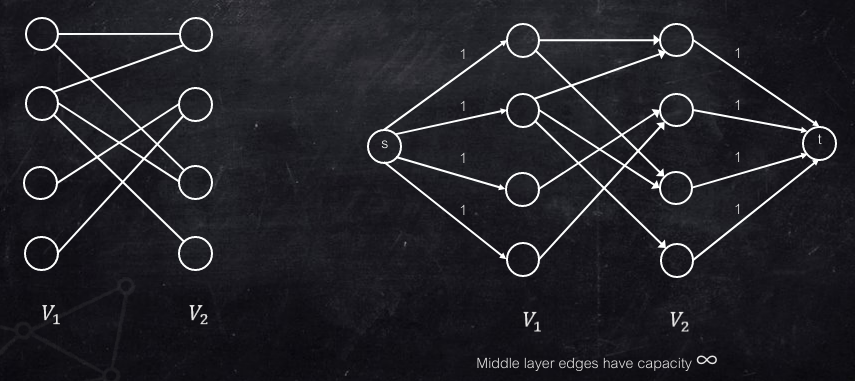
\includegraphics[width=0.5\textwidth]{fig/bipartition.png}
\end{figure} 
To solve the problem,
\begin{itemize}
	\item Find max flow in this network
	\item Recall that it will be integral
	\item Since the total capacity into each vertex in $v \in V_1$ is 1, at most one edge touching $v$ in middle layer (original bipartite graph) can carry flow out. That sounds like a matching!
	\item Similarly, since total capacity out of any vertex $v \in V_2$  is 1, at most one edge touching $w$ in middle layer can carry flow in.
	\item So, choose the matching to be all the edges in the middle layer that carry non-zero flow.
\end{itemize}

\subsection{Correctness}
\paragraph{Main Idea:} If bipartite graph has a matching of size $k$, then flow network has flow of value $k$. Conversely, if flow network has flow of value $\ell$, then there is a matching of size $\ell$. So, maximum matching corresponds to max flow value and it is what the max flow algorithm finds!

\subsubsection{Hall's theorem}
Max-flow min-cut theorem allows us to make an important observation about matching in bipartite graphs. Say a matching is perfect if it matches all vertices.

For a set of vertices $S$, define the neighborhood of $s$ as $\Gamma(S) = \{v: \exists u \in S: (u, v) \in E\}$.
\begin{theorem}
	A bipartite graph $G=(V_1 \cup V_2, E)$ has a perfect matching if and only if:
	\begin{itemize}
		\item $|V_1| = |V_2|$
		\item $\forall S \subseteq V_1, |\Gamma(S)| \ge |S|$
	\end{itemize}
\end{theorem}

\begin{proof}
	For a perfect matching to exist, the conditions of Hall's Theorem are clearly necessary. For the first condition, if the two sides have different numbers of vertices, no perfect matching can exist. For the second condition, if $|\Gamma(S)| < |S|$, vertices in $S$ cannot all be matched, which is shown in the following figure.
	\begin{figure}[H]
		\centering
		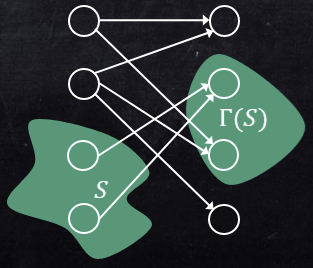
\includegraphics[width=0.3\textwidth]{fig/hall-theorem.png}
	\end{figure} 

	For the other direction, suppose for all sets $S \subseteq V_1$, $|\Gamma(S)| \ge |S|$ holds true. We will show by contradiction that the min-cut in the flow network for $G$ must have capacity $n = |V_1| = |V_2|$. Then by max-flow-min-cut theorem, the max flow will also be size of $n$. Finally, this implies that $n$ edges in middle layer are carrying flow, which means that the matching we get is of size $n$.
	
	Suppose for contradiction there is a min-cut of size less than $n$. Let's picture this situation,
	\begin{figure}[H]
	\centering
	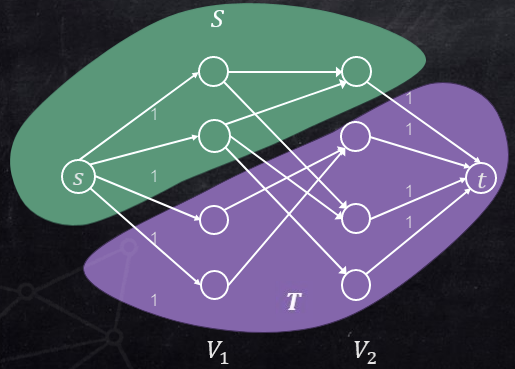
\includegraphics[width=0.3\textwidth]{fig/hall-theorem-proof.png}
	\end{figure} 	
	
	There are four sets in the graph, $S \cap V_1$, $S \cap V_2$, $T \cap V_1$, $T \cap V_2$. By observing, we get the facts that

	\begin{itemize}
		\item Edges from $s$ to $T \cap V_1$ cross the cut in forward direction with total capacity $|T \cap V_1|$.
		\item Edge from $S \cap V_2$ to $t$ cross the cut in forward direction with total capacity $|S \cap V_2|$.
		\item Other edges from $s$ and to $t$ do not cross the cut.
	\end{itemize}

	Note that none of the middle layer edges can cross the cut in the forward direction, because they have infinite capacity, and this would make the cut have infinite capacity. But a min cut will have finite capacity.
	
	Moreover, we do not care if they cross the cut in the backward direction, because such edges do not contribute to cut capacity.
	
	Therefore, the capacity of min cut = $|T \cap V_1| + |S \cap V_2|$.
	
	There are $n$ total vertices in $V_1$. They are either in $S$ or in $T$. So we can rewrite capacity as $(n- |S \cap V_1|) + |S \cap V_2|$. 
	
	Since the cut is of finite capacity, all neighbors of $S \cap V_1$ are in $S \cap V_2$. By hypothesis of hall's theorem, for any set in $V_1$, the size of its neighbor is at least as large as it is. So $|S \cap V_1| \le |S \cap V_2|$.
	
	Thus $(n- |S \cap V_1|) + |S \cap V_2| = n + (|S \cap V_2| - |S \cap V_1|) \ge n$.
	So the min cut is actually of size at least $n$, and so is the max flow value. This means the graph must have a perfect matching.
	
\end{proof}
\section{Application: Max Number of Edge-disjoint Paths in Directed Graph}
We can use network flow algorithm to find out the maximum number of edge-disjoint $s-t$ paths in a directed graph $G = (V, E)$.

The disjoint paths are paths which do not share edges. For example, there are $3$ edge-disjoint $s-t$ paths in the following figure.

\begin{figure}[H]
	\centering
	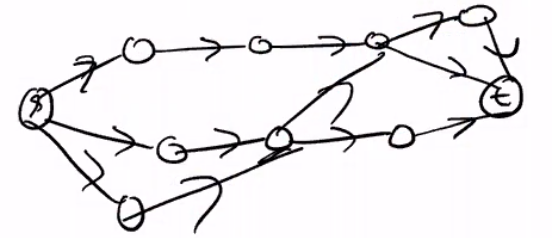
\includegraphics[width=0.5\textwidth]{fig/disjoint-path-eg.png}
\end{figure} 

How to find the largest number of such path? Set up flow network and set the capacity on each edge as 1.

\begin{theorem}
	Max flow value in this network equals max number of edge-disjoint paths from $s$ to $t$.
\end{theorem}

\begin{proof}
	It can be proved by proving two statements:
	\begin{itemize}
		\item If there are $k$ edge-disjoint paths, then there is a flow with value $k$.
		\item If max flow value is $k$, there are $k$ edge-disjoint paths.
	\end{itemize}

The first statement is easy to prove by conservation constrains. The capacity of each edge-disjoint path is $1$. Summing up $k$ of them give a flow of $k$.

For the second statement, suppose $k$ is an integer. Can assume max flow is integral. Every edge either carry 0 or 1 unit of flow. The idea is to find path one by one from the edge that carry non-zero flow.

Prove by induction on the number of edges carry non-zero flows.

\begin{itemize}
	\item Inductive state: the second statement is true for any graph with $n$ non-zero flow edges.
	\item Base case: one edge with non-zero flow. Then there is only one edge from $s$ going to $t$. The statement is obvious true since there is only one path.
	\item Inductive hypothesis: Assume that if there are $k$ edges with non-zero flow, then can find $k$ edge-disjoint paths.
	\item Inductive step: Consider a flow with $k+1$ edges with non-zero flow. 
	\begin{itemize}
		\item Case 1: Add one more edge and we reach $t$. So we find one $s-t$ path. Remove the edge from the graph. Remaining flow is a feasible flow on the remaining graph. Flow value is one less. Say original flow value was $F$. By induction, can find $F-1$ edge-disjoint path in remaining graph. Overall $F$ edge-disjoint paths.
		\item Case 2: If we get a cycle, can zero out flows on cycle. This preserve the flow value. But now the number of edges with non-zero flow $\le k$. Therefore, the theorem is true by inductive hypothesis.
	\end{itemize}
\end{itemize}
\end{proof}
\subsection{Duality Theorem}

Does the max-flow-min-cut theorem give us any additional insight here? Consider
max flow $f$, suppose there is a min-cut in the following plot. $F$ is the max flow value so $F = \#\text{ of edge-disjoint path}$. The capacity of min-cut is $F$.

\begin{figure}[H]
	\centering
	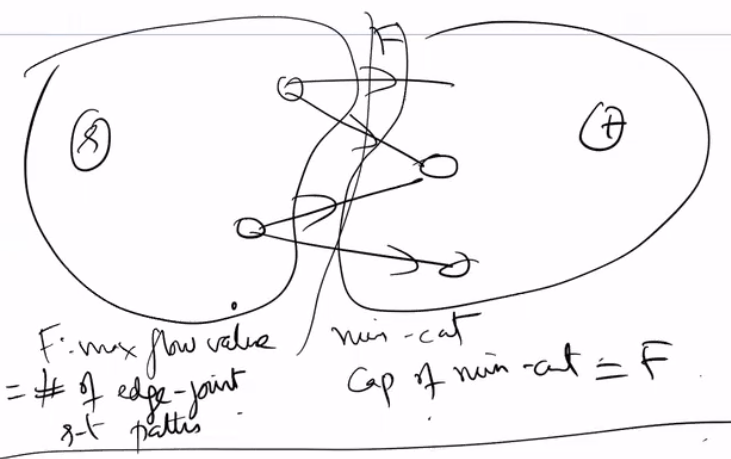
\includegraphics[width=0.5\textwidth]{fig/min-cut-eg.png}
\end{figure}

We know that the capacity of min-cut is the sum of the capacities of the forward edges. Since every edge has capacity 1, there must be $F$ forward edges for this min-cut.
 
\begin{theorem}
	(Menger's theorem 1927) If we remove $F$ edges we can disconnect $t$ from $s$. In a directed graph $G$ for any two vertices $s$, $t$, the max number of edge-disjoint $s-t$ path is equal to the minimum numbers of edges to remove to disconnect $t$ from $s$. 
\end{theorem}

\subsection{Further Extension: Undirected Graphs}
Can we find edge-disjoint paths in undirected graphs? It is easy convert undirected graph into a directed graph. So for any given $G$, $s$ and $t$, we can convert $G$ into $G'$ as a directed graph. Then put capacities as 1 on all the edges in $G'$. Then solve max flow as what we have done. 

But note that we may find edge-disjoint paths in directed graph, which may not be edge-disjoint in undirected. For example, there are two edge-disjoint path in the following graph but actually there are two edges share the same undirected edge. 

There is a quick fix for the problem, once you find the flow is carried by opposite edges then we can reduce at least one of them to zero. 
\begin{figure}[H]
	\centering
	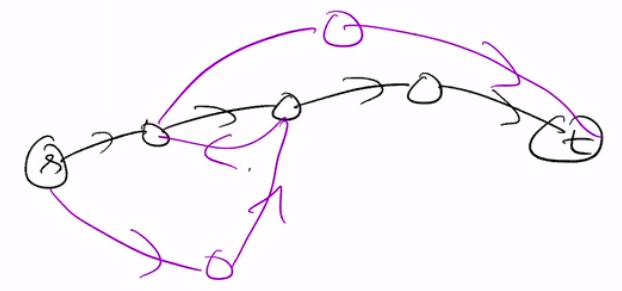
\includegraphics[width=0.5\textwidth]{fig/counter-example.png}
\end{figure}

\subsection{Further Extension: Multiple Sources and Sinks}
Think about a realistic situation: a company has many factories producing some object. Each factory can only produce a certain amount of product per day. So the supplies are available in different locations. Those produced product needs to be transported to certain distribution centers. Each distribution center has certain demands for the product. 

So what we have now is a network with multiple source and sink. Each factory is a source with certain level of supply of the product and each distribution center is a sink with certain need for the product.

Suppose each vertex $v$ has demand $d_v$. 
\begin{itemize}
	\item If $d_v > 0$, then $v$ has a demand $d_v$.
	\item If $d_v < 0$, then $v$ can supply $-d_v$.
\end{itemize}

Goal: Meet the ``demands'' at all vertices.

Necessary condition: \[\sum_{v: d_v > 0}|d_v| = \sum_{v:d_v < 0} |d_v| = D\]

Find feasible solution meaning capacity and demand conditions. Now the conservation constrain we normally have in flow has been replaced by demand conditions. We would not call the solution as a flow, instead, we call it a circulation since it does not satisfy conservation constrain anywhere.

If $v$ has demand $d_v$, \[\sum_{u: (u, v)\in E} - \sum_{u:(v, u)\in E} f(v, u) = d_v\]

The solution is simple. On the graph, have a super source and super sink in the graph $G$. For each supplier vertex with $d_v < 0$, connect an edge from the super source to it. For each distribution vertex with $d_v > 0$, connect an edge from the vertex to sink. Then the conservation constrain holds in the new graph and we can solve max-flow in the network. The max-flow is at most $D$. In fact, the max-flow needs to be $D$ in order to satisfy all demands.

If max-flow less than $D$, no feasible circulation. Otherwise, output is the answer.

\subsubsection{Further Extension: Capacities and Lower Bound Constrains}
Sometimes we would like to add some constrains at edge $e \in E$:
\begin{itemize}
	\item $f(e) \ge l(e)$
	\item $f(e) \le c(e)$
\end{itemize}

We can reduce this problem to a flow problem. First put lower bound amount of flow on each edge. Create a flow $f$, for each edge $e$, $f(e) = l(e)$. Doesn't satisfy conservation constrain.

Find a flow $f'$ to augment $f$. Final solution will be $f+f'$. $f'$ needs to re-establish conservation at all vertices besides $s$ and $t$. 

Let $d_v = \sum_{u} f(v, u) - \sum_u f(u, v)$. The capacity of each edge $e: c_e - l_e$. Find a circulation $f'$ in network with above demands and above capacities.

A feasible circulation solves the problem of finding a flow that satisfies both lower bound and capacity constrains.













\end{document}
